\chapter{Alberi}
Un albero è un grafo connesso senza cicli, ovvero un DAG connesso. Una delle caratteristiche 
fondamentali degli alberi è che essi hanno esattamente $n-1$ archi, proprietà che può essere
proposta anche per un grafo connesso senza cicli ricordando che il numero $n$ di nodi che costituiscono 
un albero può essere inteso come $|V|$, dove $V$ è l’insieme dei vertici del grafo $G$. Dunque
per verificare che un grafo non abbia cicli è sufficiente stabilire che abbia un numero di archi
pari a $n-1$. In questo caso, essendo fornito un grafo semplice e connesso con $n$ nodi ed $m$ archi
basta implementare un algoritmo che verificare che $m = n-1$, ovvero effettuare un confronto
semplice con costo costante $O(1)$.
\section{Tipi di albero}
\textbf{Albero libero:} Un albero libero è un tipo di grafo non orientato connesso e senza cicli, 
ovvero un DAG (Directed Acyclic Graph) connesso. Non è caratterizzato da uno specifico nodo 
che assume il ruolo di radice, bensì qualsiasi nodo può esserlo.\medskip\\
\textbf{Albero radicato:} Un albero radicato è una tipologia di albero libero in cui un vertice è 
stato scelto come radice. La radice è il punto di partenza da cui si può raggiungere ogni altro nodo attraverso 
un percorso unico.\medskip\\
\textbf{Albero ordinato:} Un albero radicato si dice \textbf{ordinato} se i figli di ogni nodo hanno un ordine specifico. 
Inoltre l'ordine può essee necessario per la visita pre-ordine, in-ordine e post-ordine.\medskip\\
\textbf{Albero posizionale:} Un. albero ordinato si dice posizionale se ad ogni figlio di un nodo è associata 
una posizione specifica, ad esempio quando si parla di figlio "destro" e "sinistro" per gli alberi binari. Ricorda: le posizioni sono 
etichettate e differenziano i figli di un nodo. Quando non sono occupate da un nodo sono posizioni vuote.\medskip\\
\textbf{Albero k-ario:} Un albero $k$-ario è un albero posizionale in cui ogni posizione maggiore di
$k$ è vuota, ciò si traduce nel dire che ogni nodo ha al massimo $k$ figli. Viene utilizzato per
rappresentare strutture con una quantità fissa di sottoelementi.\medskip\\
\textbf{Albero binario:} Un albero binario è un esempio di albero $k$-ario in cui ogni nodo ha al
massimo due figli, pertanto $k = 2$. I due figli sono tipicamente chiamati ”destro” e ”sinistro”.
Questa tipologia di albero è fondamentale per molte strutture dati e algoritmi, come gli alberi
binari di ricerca e gli heap.
\section{Alberi binari}
\subsection{Rappresentazione degli alberi binari}
Ogni nodo dell'albero è composto dai seguenti attributi:
\begin{enumerate}
    \item Puntatore al nodo padre \textbf{p}
    \item Puntatore al figlio sinistro \textbf{l}
    \item Puntatore al figlio destro \textbf{r}
    \item Chiave del nodo \textbf{key}, ovvero l'attributo in cui viene memorizzata l'etichetta del nodo
\end{enumerate}
\noindent \subsection{Albero binario di ricerca BST}
Un albero di ricerca definito con la sigla BST, è un albero binario che soddisfa la seguente proprietà:
\begin{definition}
   Sia $x$ un nodo di un albero di ricerca, se $y$ è un nodo del sottoalbero sinistro di $x$ allora 
   $y.key \le x.key$, mentre se $y$ è un nodo del sottoalbero destro di $x$ allora $y.key \ge x.key$  
\end{definition}
\subsection{Visita di un albero binario}
Diversamente dal caso delle strutture lineari, dove è possibile visitare tutti gli elementi in
sequenza nell’ordine in cui sono rappresentati, nel caso di alberi binari vi sono modi diversi
di esplorare i nodi. In particolare, le tre operazioni caratteristiche della visita in profondità
(visita della radice, visita del sottoalbero sinistro, visita del sottoalbero destro) possono essere
realizzate in qualunque ordine. Esistono tre versioni di visita in profondità:
\begin{enumerate}
    \item \textbf{Attraversamento simmetrico o visita in ordine (inorder tree walk):} sottoalbero sinistro, 
    radice, sottoalbero destro. Ciò implica che i nodi vengono visitati in ordine crescente di chiave.
    \item \textbf{Attraversamnto anticipato (preorder tree walk):} radice, sottoalbero sinistro,  sottoalbero destro. 
    Ciò implica che la radice venga visitata prima dei suoi sottoalberi.
    \item \textbf{Attraversamento posticipato (postorder tree walk):} sottoalbero sinistro, sottoalbero destro, radice. 
    \item Ciò implica che la. radice venga visitata dopo dei suoi sottoalberi. 
\end{enumerate}
\begin{verbatim}
    Pre-order(x){
        if x != nil
            print x.key
            Preorder(x.left)
            Preorder(x.right)
    }
    Post-order(x){
        if x != nil
            Postorder(x.left)
            Postorder(x.right)
            print x.key
    }
    In-order(x){
        Inorder(x.left)
        print x.key
        Inorder(x.right)
    }
\end{verbatim}
\subsection{Analisi della complessità}
\colorbox{SALZO}{\parbox{\dimexpr\linewidth-2\fboxsep}{\begin{theorem}
Se $x$ è la radice di un sottoalbero con $n$ nodi allora \textbf{Inorder(x)} richiede un tempo $\mathbf{\Theta(n)}$
\end{theorem}}}
\begin{proof}
Sia $T(n)$ il tempo richiesto è $\Omega(n)$ e allo stesso tempo $O(n)$.\\
Dire che $T(n)$ è $\Omega(n)$ significa che $T(n)$ è almeno pari a $c \cdot n$ per qualche costante $c$ e per $n$ 
sufficientemente grande. Durante l'attraversamento in-ordine dobbiamovisitare tutti i nodi, ogni nodo deve essere 
visitato almeno una volta, ecco spiegato il motivo per il quale il tempo richiesto per visitare tutti i nodi è almeno proporzionale ad $n$.\\
Dire che $T(n)$ è $O(n)$ significa che $T(n)$ è al massimo $c \cdot n$ per qualche costante $c$ e per $n$ sufficientemente grande. Sapendo che l'algorimto 
di attraversamento in-ordine segue questi passi:
\begin{enumerate}
    \item Visita il sottoalbero sinistro
    \item Visita la radice $x$
    \item Visita il sottoalbero destro
\end{enumerate}
\noindent Supponiamo che $n=0$, per visitare un nodo serve una piccola quantità di tempo, basta verificare che $x=nil$, ecco perchè $T(n=0)=c$.\\
Supponendo che $n>0$ e che il sottoalbero sinistor abbia k nodi e il sottoalbero destro ne abbia $n-k-1$, il tempo totale $T(n)$ è quindi minore o uguale alla somma 
dei tempi richiesti per visitare il sottoalbero sinistro, la radice e il destro:\\
$$T(n) \le T(k) + T(n-k-1)+d $$\\
dove $d$ è il tempo costante per visitare la radice $x$ (che è un'operazione. $O(1)$). Applichiamo il metodo di sostituzione per dimostrare che:\\
$$T(n)=(c+d)n+c$$ per ogni $n \ge 0$\\
\textbf{CAso base (n==0):} $T(0)=c=(c+d) \cdot 0 + c$\\
\textbf{Per n$>$0}:\\
$T(n) \le T(k) + T(n-k-1)+d$
$=((c+d)k+c)+((c+d)(n-k-1)+c)+c$\\
$=(c+ d)k+ c+ (c+ d)n-(c+ d)k-(c+ d) + c+ d$\\
$= c-c-d+ d+ c+ (c+ d)n$\\
$= (c+ d)n+ c$
\end{proof}
\subsection{Interrogazioni di un albero binario di ricerca}
I BST sono strutture dati. sulle quali vengono realizzate molte delle operazioni definite su insiemi dinamici, anche chiamate "interrogazioni"
\begin{enumerate}
    \item \textbf{Search(x, key):} data la radice $x$ e una chiave key, restituisce il puntatore a un nodo con chiave key, se esiste, o nil
    \item \textbf{Minium(x) o Maxium(x):} dato un albero con radice $x$, restituisce l'elemento la cui chiave è minima o massima
    \item \textbf{Successor(x) o Predecessor(x):} dato un albero con radice $x$, restituisce il nodo successivo o precedente a $x$ rispetto all'attraversamento simmetrico
\end{enumerate}
\noindent \begin{verbatim}
    Search(x, k){
        if x == nil or k == x.key
            return x
        if x < x.key 
            return Search(x.left,  k)
        else
            return Search(x.right, k)
    }
    Minimum(x){
        while x.right 1 nil
            x = x.right
        return x
    }
    Maximum(x){
        while x.right 1 nil
            x = x.right
        return x
    }
    Successor(x){
        if x.right != nil
            return Minimum(x.right)
        else 
        y = x.p
        while y != nil and x == y.right
            x = y
            y = x.p 
        return y
    }
    Predecessor(x){
        if x.left != nil
            return Maximum(x.left)
        else 
        y = x.p
        while y != nil and x == y.left
            x = y
            y = x.p 
        return y
    }
\end{verbatim}
\noindent Tutte queste funzioni hanno costo \textbf{O(h)}, dove $h$ è l'altezza del nodo $x$ nell'albero.  \medskip\\
Tra queste vi è una categoria ”a parte” che riguarda le operazioni che agendo sull’albero ne
modificano il contenuto. Nel caso di alberi binari di ricerca queste operazioni devono essere
realizzate preservando la proprietà dell’ordinamento delle chiavi. Ciò significa che è necessario
 verificare se un inserimento o cancellazione interferiscono con tale proprietà, in tal caso è
necessario aggiornare l’albero affinchè sia possibile ripristinarla.
\begin{enumerate}
    \item \textbf{Insert(T,z):} l'idea è quella di inserire nell'albero un nuovo nodo z sottoforma di foglia. Affonchè ciò 
    sia possibile, è necessario trovare una foglia che possa diventare per essa il padre senza compromettere le proprietà dell'albero
    \item \textbf{Delete(T, z):} il ragionamento per questo tipo di operazione non è unico, bensì ci si può trovare in tre situazioni diverse: 
    \begin{itemize}
        \item \textbf{z è una foglia}, ovvero non ha filgi: si elimina il nodo modificando a nil il puntatore del padre
        \begin{figure}[H]
            \centering  
            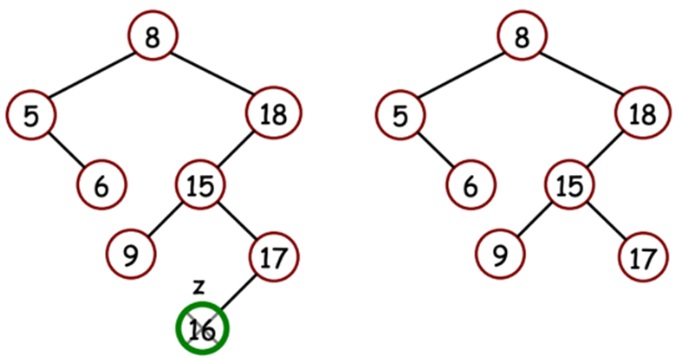
\includegraphics[width=0.6\linewidth]{../images/delete1_alberi.png}
        \end{figure}
        \item \textbf{z ha un figlio, w:} in tal caso è come se il nodo $w$ venisse "promosso" a prendere il posto di $z$ nell'albero, aggiornando il 
        puntatore del padre di $z$ in modo che punti a $w$
        \begin{figure}[H]
            \centering  
            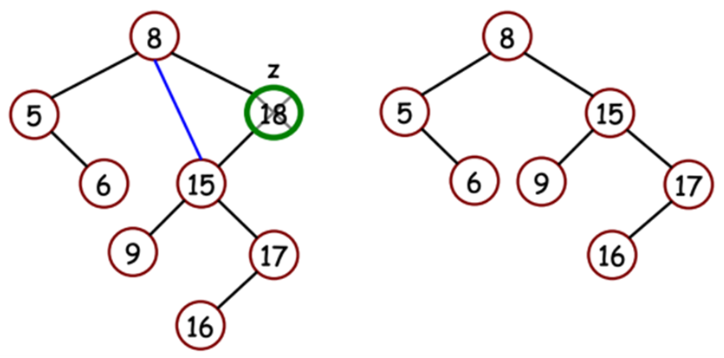
\includegraphics[width=0.6\linewidth]{../images/delete2_alberi.png}
        \end{figure}
        \item \textbf{z ha due figli:} bbisogna trovare il successore $y$ di z nel sottoalbero destro, spostare
$y$ nella posizione precedentemente coperta da z, infine ricollegare i sottoalberi. Per
spostare y bisogna tener conto di una condizione, ovvero se $y$ è figlio destro di z
semplicemente lo si fa risalire per poi “attaccargli” il vecchio sottoalbero sinistro di
z, altrimenti si scambia $y$ con il suo figlio destro per poi portare verso l’alto $y$ fino a
sostituire z
    \end{itemize}
    \begin{figure}[H]
            \centering  
            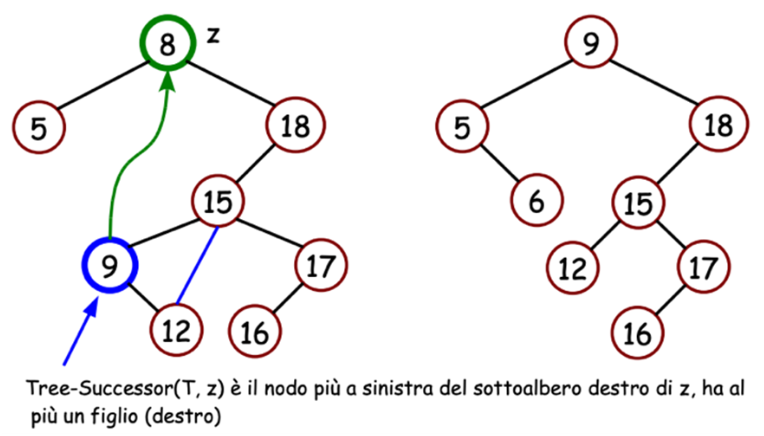
\includegraphics[width=0.6\linewidth]{../images/delete3_alberi.png}
        \end{figure}
\end{enumerate}
\noindent \textbf{Pseudocodice}
\begin{verbatim}
    Insert(T, z){
        x = T.root
        y = nil
        while x!= NULL //trovo nodo dove attccare z
            y = x
            if z.key < y.key
                x = y.left
            else
                x = y.right
        z.p = y
        
        if y == nil // l’ albero e’ vuoto
            T.root = z // z diventa la radice
        else if z.key < y.key // inserisco z nell ’ albero
            y.left = z
        else
            y.right = z
    }

    Transplant(T, u, v){
        if u.p == nil
            T.root = v
        else if u == u.p.left
            u.p.left = v
        else
            u.p.right = v
        if v != nil
            v.p = u.p
    }

    Delete(T, z){
        if z.left == nil
            // se il sottoalbero sinisto di z e’ vuoto, devo attaccare z. right a z.p
            Transplant(T, z, z. right)
        else if z.right == nil
            // se il sottoalbero destro di z e’ vuoto, devo attaccare z. left a z.p
            Transplant(T, z, z. left )
        // cosi facendo ho trattato i casi se z ha un solo figlio oppure e’ una foglia
        else
            y = Minimum(z.right) // trovo y, il successore di z
            // sposto y nella posizione di z, tenendo conto dei sottoalberi di y
            if y != z.right
                Transplant(T, y, y.right)
                y.right = z.right
                y.right.p = y  
            Transplant(T, z, y)
                y.left = z.left
                y.left.p = y
    }
\end{verbatim}
\noindent Costo $\mathbf{O(h)}$, dove $h$ è l'altezza dell'albero.\\
\textbf{SE CE METTERE ESEMPIO INSERT DAL LIBRO}
\section{Alberi Rosso-Neri}
Un albero rosso-nero è un albero binario di ricerca con un bit in più di memoria per ogni nodo
necessario per il colore, che può essere RED o BLACK. L’albero si dice \textbf{approssimativamente
bilanciato} poichè, grazie a specifici vincoli per assegnare i colori ai nodi, garantisce che nessun
cammino che va dalla radice a una foglia sia lungo più del doppio di qualsiasi altro.
Ogni nodo ha i seguenti attributi: color, key, left, right e p. Se manca un figlio o il padre di
un nodo, il corrispondente attributo puntatore del nodo contiene il valore NIL, il quale viene
trattato come un puntatore a una foglia.\\
\subsection{Proprietà di un albero rosso-nero}
\begin{enumerate}
    \item Ogni nodo è rosso o nero
    \item La radice è nera 
    \item Ogni foglia (NIL) è nera 
    \item Se unnodo è rosso, allora entrambi i suoi figli sono neri 
    \item Per ogni nodo, tutti i cammini semplici che vanno dal nodo alle foglie sue discendenti cotengono 
    lo stesso numero di nodi neri
    \item L'altezza massima di un albero rosso-nero con $n$ nodi interni è $2 \cdot \log(n+1)$
\end{enumerate}
\begin{figure}[H]
    \centering  
    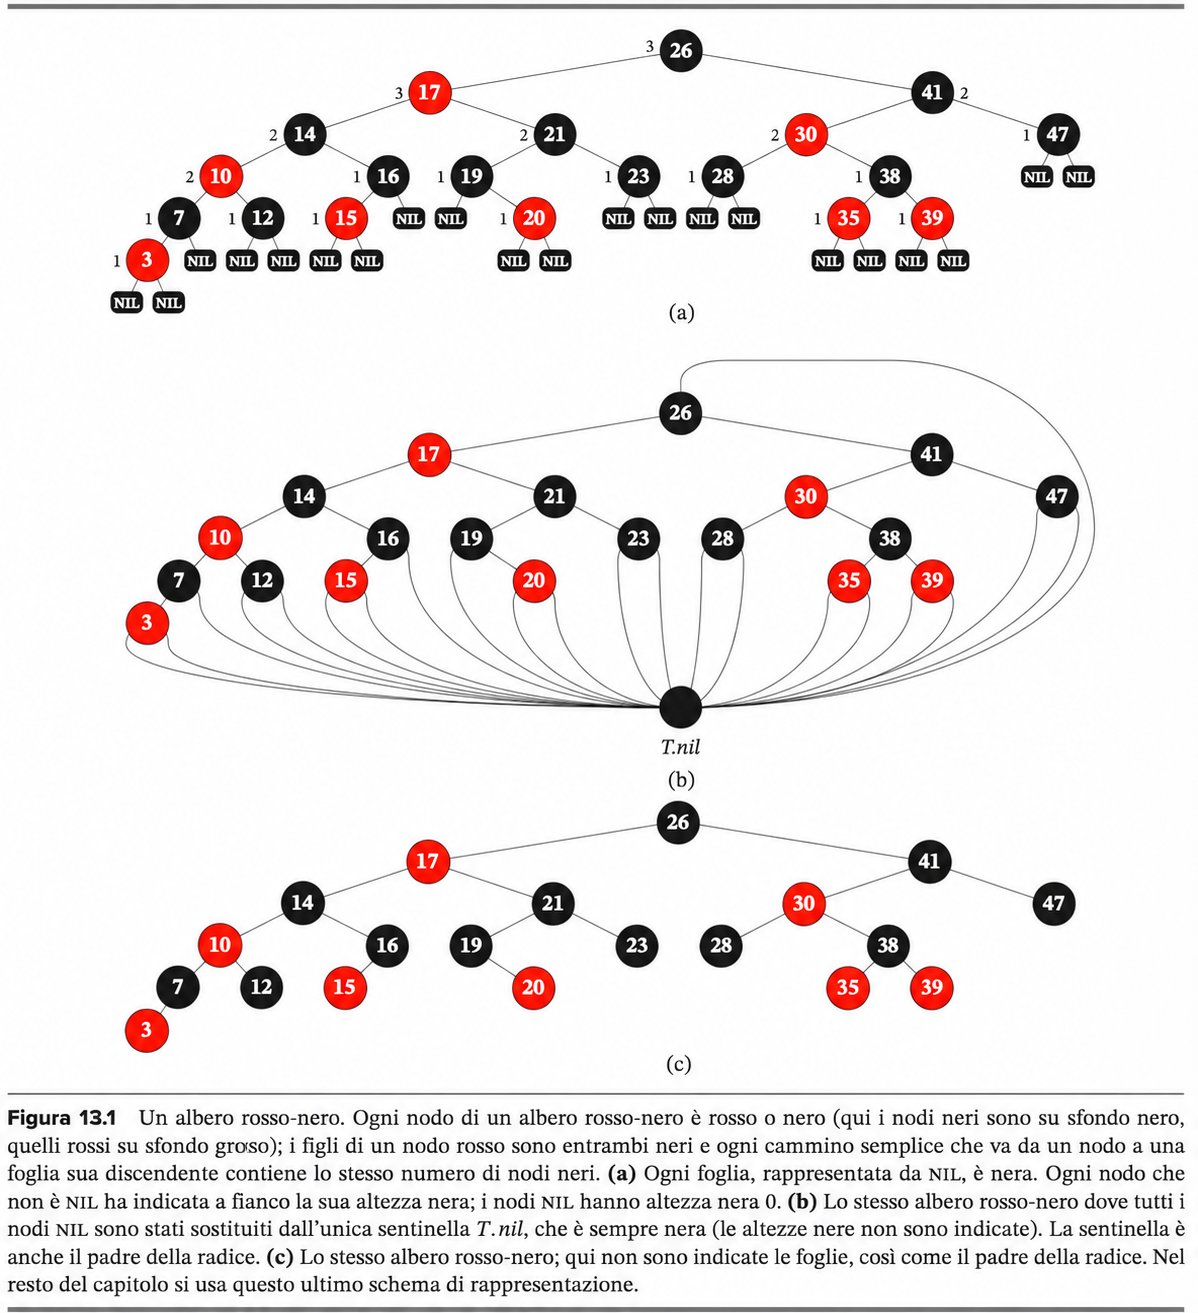
\includegraphics[width=0.9\linewidth]{../images/alberi_rosso_neri.png}
\end{figure}
\noindent Per un albero rosso-nero si definisce sentinella, l’oggetto $T.nil$ con gli stessi attributi di un nodo
ordinario dell’albero, il suo colore è ”BLACK” e gli attributi p, left, right e key possono assumere
valori arbitrari. Bisogna notare che tutti i puntatori a $NIL$ sono sostituiti con puntatori alla
sentinella. L’uso di quest’ultima permette di trattare un figlio $NIL$ di un nodo $x$ come un nodo
ordinario il cui padre è $x$.
Si definisce altezza nera di un nodo $x$, indicata da $\mathbf{bh(x)}$, il numero di nodi neri lungo un
cammino semplice che inizia dal nodo $x$ (ma non lo include) e finisce in una foglia. La Proprietà
$5$ permette di definire questo concetto, infatti tutti i cammini semplici che scendono dal nodo
hanno lo stesso numero di nodi neri. Per definizione, l’altezza nera di un albero rosso-nero è
l’altezza nera della sua radice.\\
\textbf{VEDERE ULTIME DEFINZIONI SULLE SLIDE E RISCRIVERLE}